\chapter{Streamlines}

\modinfo{Directory}{FlowStreamlines}
\modinfo{Solvers}{\Idx{StreamSolver}, \Idx{FlowSolve}}
\modinfo{Tools}{\Idx{ElmerGrid}, editor}
\modinfo{Dimensions}{2D}

\subsection*{Case definition}
The case definition is the same as in the incompressible flow passing a step.
The mathematical definition of the stream function $\psi$ is
\begin{equation}
u \, = \, \frac{\partial \psi}{\partial y} \, , \quad
v \, = \, - \frac{\partial \psi}{\partial x} \,.
\end{equation}
where $u,v$ are the velocity components in $x,y$ geometry.
For more info check Elmer Models Manual.

\subsection*{Solution Procedure}
First we create a mesh with ElmerGrid. The mesh is defined in
{\tt step.grd} and it is created with command
\ttbegin
ElmerGrid 1 2 step
\ttend
You may need to compile the StreamSolver yourself. If the Elmer environment is 
successfully setup the compilation command should look like
the following lines, 
\ttbegin
elmerf90 -o StreamSolver StreamSolver.f90
\ttend
The solver input file {\tt streamlines.sif} starts with 
the definition of the mesh directory. 
\ttbegin
Header
  Mesh DB "." "step"
End
\ttend
The simulation uses 2D Cartesian geometry and searches a Steady State.
There is no coupled solvers so only one iteration is needed. 
Numerical results are written to file {\tt streamlines.result}
and ElmerPost file is {\tt streamlines.ep}.
\ttbegin
Simulation
  Coordinate System =  Cartesian 2D
  Coordinate Mapping(3) = 1 2 3

  Simulation Type = Steady
  Steady State Max Iterations = 1

  Output Intervals = 1
  Post File = "streamlines.ep"
  Output File = "streamlines.result"
End
\ttend
There is just one body and it uses equation 1 and
is of material 1.
\ttbegin
Body 1
  Equation = 1
  Material = 1
End
\ttend
The equation block states that we use Solvers 1 and 2 to solve the problem
and that we use Navier-Stokes equations.
\ttbegin
Equation 1
  Active Solvers(2) = 1 2
  Navier-Stokes = True
End
\ttend
In material block we define the density and the viscosity of the fluid.
\ttbegin
Material 1
  Density = 1
  Viscosity = 0.01
End
\ttend
Solver 1 is for the Navier-Stokes equations.
Here we give the linear system solver
\footnote{Biconjugate gradient method with incomplete LU preconditioning}
and convergence criterions for linear, nonlinear and steady state 
solution of the Navier-Stokes equations.
\ttbegin
Solver 1
  Equation = "Navier-Stokes"
  Stabilize = True

  Linear System Solver = Iterative
  Linear System Iterative Method = BiCGStab
  Linear System Max Iterations = 500
  Linear System Convergence Tolerance = 1.0e-8
  Linear System Preconditioning = ILU1

  Nonlinear System Convergence Tolerance = 1.0e-6
  Nonlinear System Max Iterations = 15
  Nonlinear System Newton After Iterations = 8
  Nonlinear System Newton After Tolerance = 1.0e-4
  Nonlinear System Relaxation Factor = 1.0

  Steady State Convergence Tolerance = 1.0e-6
End
\ttend
Then the solver for streamlines.
\begin{itemize}
\item Name of the equation. This may be what ever you like.
\item Name of the binary file and the subroutine. If you compiled the StreamSolver yourself,
then you may need to change this to \texttt{Procedure = "./StreamSolver" "StreamSolver"}.
\item Name of the variable. This may be what ever you like.
\item Stream function is scalar, so the degree of freedom is 1.
\end{itemize}
Next set of keywords is for the StreamSolver. More info on keywords is in the Elmer
Models Manual.
\begin{itemize}
\item Name of the flow field variable. The name of the FlowSolves variable is FlowSolution.
\item Global number of the offset node. 1 is always a safe choice.
\item Shift the smallest value to zero.
\item Scale the maximum value to 1.
\item Use the normal stream function i.e. don't use Stokes stream function.
\end{itemize}
Then we define the linear system solver and convergence criterions.
\ttbegin
Solver 2
  Equation = "StreamSolver"
  Procedure = "StreamSolver" "StreamSolver"
  Variable = "StreamFunction"
  Variable DOFs = 1

  Stream Function Velocity Variable = String "Flow Solution"
  Stream Function First Node = Integer 1
  Stream Function Shifting = Logical TRUE
  Stream Function Scaling = Logical TRUE
  Stokes Stream Function = Logical FALSE

  Linear System Solver = Iterative
  Linear System Iterative Method = BiCGStab
  Linear System Max Iterations = 500
  Linear System Convergence Tolerance = 1.0e-8
  Linear System Preconditioning = ILU1

  Steady State Convergence Tolerance = 1.0e-6
End  
\ttend
Finally we give the boundary conditions.
The condition 1 is for the lower and upper side of the step 
($\Gamma_1$,$\Gamma_2$,$\Gamma_3$,$\Gamma_5$ in case definition).
Here both velocities are zero.
The condition 2 is for the output edge ($\Gamma_4$). Here vertical velocity is zero. 
The condition 3 is for the input edge ($\Gamma_6$). Here horizontal velocity is 1 and 
vertical velocity is zero.
\ttbegin
Boundary Condition 1
  Target Boundaries = 1
  Velocity 1 = 0
  Velocity 2 = 0
End

Boundary Condition 2
  Target Boundaries = 2
  Velocity 2 = 0
End

Boundary Condition 3
  Target Boundaries = 3
  Velocity 1 = 1
  Velocity 2 = 0
End
\ttend
\subsection*{Results}
Problem is solved with command {\tt Solver}. The results are then viewed with
ElmerPost. In figure~\ref{f:streamlines} are some contour lines of the stream
function. These are also flows streamlines. The contour values are manually
selected to get a nice picture. Note the swirl after the step.
\begin{figure}[!hb]
\begin{center}
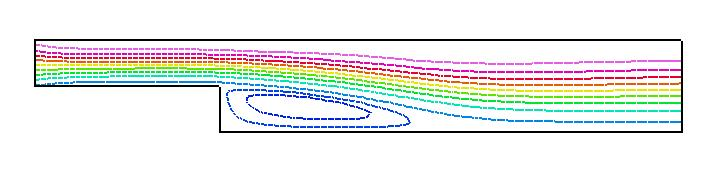
\includegraphics[width=1.0\textwidth]{lines}
\end{center}
\caption{The streamlines of the flow.}
\label{f:streamlines}
\end{figure}







